% Source of fig_switch_kink.pdf (Figure 1 in manuscript_neurocomputing_journal_cas_dc.tex).
% Standalone document: compile separately; NOT part of the main compilation.
% To regenerate: pdflatex fig_switch_kink.tex
\documentclass[border=2pt]{standalone}
\usepackage{amsmath,amssymb}
\usepackage{xcolor}
\usepackage{pgfplots}
\pgfplotsset{compat=1.17}
\usepgfplotslibrary{groupplots}
\newcommand{\relu}{\sigma}
\begin{document}
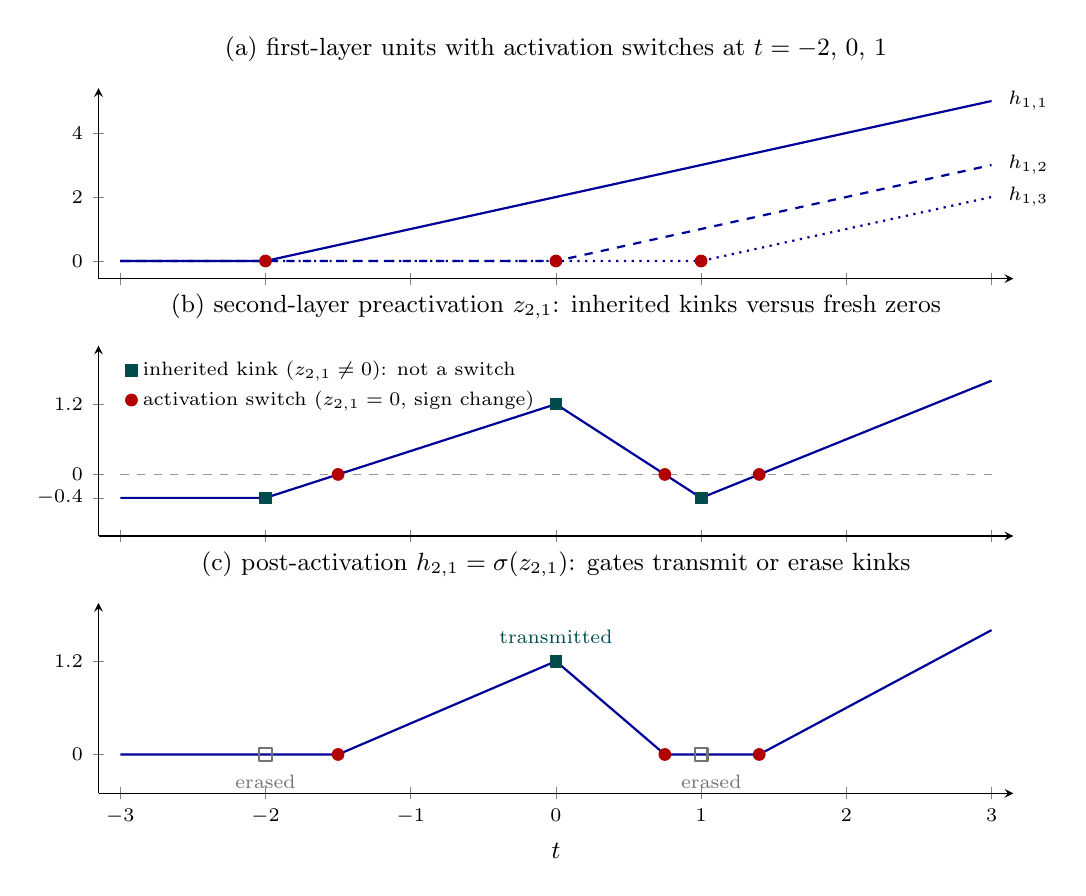
\begin{tikzpicture}[
  line join=round,
  swmark/.style={only marks, mark=*, mark size=2.1pt, color=red!70!black},
  inhmark/.style={only marks, mark=square*, mark size=2.1pt, color=teal!60!black},
  gonemark/.style={only marks, mark=square, mark size=2.3pt, color=black!55, thick}
]
\begin{groupplot}[
  group style={group size=1 by 3, vertical sep=0.85cm, xticklabels at=edge bottom},
  width=13.2cm, height=4.0cm,
  xmin=-3.15, xmax=3.15,
  xtick={-3,-2,-1,0,1,2,3},
  tick label style={font=\scriptsize},
  title style={font=\small},
  axis lines=left,
  clip=false
]
\nextgroupplot[
  title={(a) first-layer units with activation switches at $t=-2,\,0,\,1$},
  ymin=-0.55, ymax=5.4, ytick={0,2,4}
]
\addplot[blue!60!black, thick] coordinates {(-3,0) (-2,0) (3,5)};
\addplot[blue!60!black, thick, dashed] coordinates {(-3,0) (0,0) (3,3)};
\addplot[blue!60!black, thick, dotted] coordinates {(-3,0) (1,0) (3,2)};
\addplot[swmark] coordinates {(-2,0) (0,0) (1,0)};
\node[font=\scriptsize, anchor=west] at (axis cs:3.05,5) {$h_{1,1}$};
\node[font=\scriptsize, anchor=west] at (axis cs:3.05,3) {$h_{1,2}$};
\node[font=\scriptsize, anchor=west] at (axis cs:3.05,2) {$h_{1,3}$};

\nextgroupplot[
  title={(b) second-layer preactivation $z_{2,1}$: inherited kinks versus fresh zeros},
  ymin=-1.05, ymax=2.2, ytick={-0.4,0,1.2},
  legend style={font=\scriptsize, at={(0.02,0.98)}, anchor=north west, draw=none, fill=none, legend cell align=left}
]
\addplot[black!40, dashed, thin, forget plot] coordinates {(-3,0) (3,0)};
\addplot[blue!60!black, thick, forget plot] coordinates {(-3,-0.4) (-2,-0.4) (0,1.2) (1,-0.4) (3,1.6)};
\addplot[inhmark] coordinates {(-2,-0.4) (0,1.2) (1,-0.4)};
\addlegendentry{inherited kink ($z_{2,1}\ne0$): not a switch}
\addplot[swmark] coordinates {(-1.5,0) (0.75,0) (1.4,0)};
\addlegendentry{activation switch ($z_{2,1}=0$, sign change)}

\nextgroupplot[
  title={(c) post-activation $h_{2,1}=\relu(z_{2,1})$: gates transmit or erase kinks},
  ymin=-0.5, ymax=1.95, ytick={0,1.2}, xlabel={$t$},
  xlabel style={font=\small}
]
\addplot[blue!60!black, thick] coordinates {(-3,0) (-1.5,0) (0,1.2) (0.75,0) (1.4,0) (3,1.6)};
\addplot[swmark] coordinates {(-1.5,0) (0.75,0) (1.4,0)};
\addplot[inhmark] coordinates {(0,1.2)};
\addplot[gonemark] coordinates {(-2,0) (1,0)};
\node[font=\scriptsize, color=black!55, anchor=north] at (axis cs:-2,-0.14) {erased};
\node[font=\scriptsize, color=black!55, anchor=north] at (axis cs:1.07,-0.14) {erased};
\node[font=\scriptsize, color=teal!60!black, anchor=south] at (axis cs:0,1.3) {transmitted};
\end{groupplot}
\end{tikzpicture}
\end{document}
